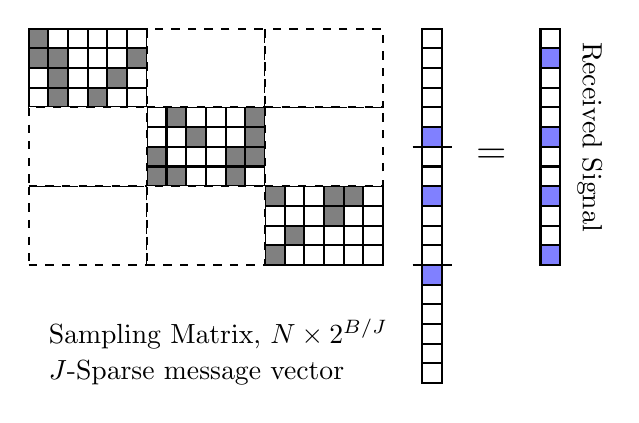
\begin{tikzpicture}
[draw=black, line width=0.75pt,
block/.style={rectangle, draw, fill=white, inner sep=0pt, minimum width=15mm,minimum height=10mm},
entry1/.style={rectangle, draw, fill=gray, inner sep=0pt, minimum size=2.5mm},
entry0/.style={rectangle, draw, fill=white, inner sep=0pt, minimum size=2.5mm},
symbol0/.style={rectangle, draw, fill=white, inner sep=0pt, minimum size=2.5mm},
symbol1/.style={rectangle, draw, fill=blue!50, inner sep=0pt, minimum size=2.5mm}]

\node[entry1] (m1800) at (4.50,0) {};
\node[entry0] (m1900) at (4.75,0) {};
\node[entry0] (m2000) at (5.00,0) {};
\node[entry0] (m2100) at (5.25,0) {};
\node[entry0] (m2200) at (5.50,0) {};
\node[entry0] (m2300) at (5.75,0) {};

\node[entry0] (m1801) at (4.50,0.25) {};
\node[entry1] (m1901) at (4.75,0.25) {};
\node[entry0] (m2001) at (5.00,0.25) {};
\node[entry0] (m2101) at (5.25,0.25) {};
\node[entry0] (m2201) at (5.50,0.25) {};
\node[entry0] (m2301) at (5.75,0.25) {};

\node[entry0] (m1802) at (4.50,0.50) {};
\node[entry0] (m1902) at (4.75,0.50) {};
\node[entry0] (m2002) at (5.00,0.50) {};
\node[entry1] (m2102) at (5.25,0.50) {};
\node[entry0] (m2202) at (5.50,0.50) {};
\node[entry0] (m2302) at (5.75,0.50) {};

\node[entry1] (m1803) at (4.50,0.75) {};
\node[entry0] (m1903) at (4.75,0.75) {};
\node[entry0] (m2003) at (5.00,0.75) {};
\node[entry1] (m2103) at (5.25,0.75) {};
\node[entry1] (m2203) at (5.50,0.75) {};
\node[entry0] (m2303) at (5.75,0.75) {};

\node[entry1] (m1204) at (3.00,1.00) {};
\node[entry1] (m1304) at (3.25,1.00) {};
\node[entry0] (m1404) at (3.50,1.00) {};
\node[entry0] (m1504) at (3.75,1.00) {};
\node[entry1] (m1604) at (4.00,1.00) {};
\node[entry0] (m1704) at (4.25,1.00) {};

\node[entry1] (m1205) at (3.00,1.25) {};
\node[entry0] (m1305) at (3.25,1.25) {};
\node[entry0] (m1405) at (3.50,1.25) {};
\node[entry0] (m1505) at (3.75,1.25) {};
\node[entry1] (m1605) at (4.00,1.25) {};
\node[entry1] (m1705) at (4.25,1.25) {};

\node[entry0] (m1206) at (3.00,1.50) {};
\node[entry0] (m1306) at (3.25,1.50) {};
\node[entry1] (m1406) at (3.50,1.50) {};
\node[entry0] (m1506) at (3.75,1.50) {};
\node[entry0] (m1606) at (4.00,1.50) {};
\node[entry1] (m1706) at (4.25,1.50) {};

\node[entry0] (m1207) at (3.00,1.75) {};
\node[entry1] (m1307) at (3.25,1.75) {};
\node[entry0] (m1407) at (3.50,1.75) {};
\node[entry0] (m1507) at (3.75,1.75) {};
\node[entry0] (m1607) at (4.00,1.75) {};
\node[entry1] (m1707) at (4.25,1.75) {};

\node[entry0] (m0608) at (1.50,2.00) {};
\node[entry1] (m0708) at (1.75,2.00) {};
\node[entry0] (m0808) at (2.00,2.00) {};
\node[entry1] (m0908) at (2.25,2.00) {};
\node[entry0] (m1008) at (2.50,2.00) {};
\node[entry0] (m1108) at (2.75,2.00) {};

\node[entry0] (m0609) at (1.50,2.25) {};
\node[entry1] (m0709) at (1.75,2.25) {};
\node[entry0] (m0809) at (2.00,2.25) {};
\node[entry0] (m0909) at (2.25,2.25) {};
\node[entry1] (m1009) at (2.50,2.25) {};
\node[entry0] (m1109) at (2.75,2.25) {};

\node[entry1] (m0610) at (1.50,2.50) {};
\node[entry1] (m0710) at (1.75,2.50) {};
\node[entry0] (m0810) at (2.00,2.50) {};
\node[entry0] (m0910) at (2.25,2.50) {};
\node[entry0] (m1010) at (2.50,2.50) {};
\node[entry1] (m1110) at (2.75,2.50) {};

\node[entry1] (m0611) at (1.50,2.75) {};
\node[entry0] (m0711) at (1.75,2.75) {};
\node[entry0] (m0811) at (2.00,2.75) {};
\node[entry0] (m0911) at (2.25,2.75) {};
\node[entry0] (m1011) at (2.50,2.75) {};
\node[entry0] (m1111) at (2.75,2.75) {};

\node[block,dashed] at (2.125,0.375) {};
\node[block,dashed] at (2.125,1.375) {};
\node[block,dashed] at (3.625,0.375) {};
\node[block,dashed] at (3.625,2.375) {};
\node[block,dashed] at (5.125,1.375) {};
\node[block,dashed] at (5.125,2.375) {};

\node[symbol0] (s07) at (6.5,-1.50) {};
\node[symbol0] (s08) at (6.5,-1.25) {};
\node[symbol0] (s09) at (6.5,-1.00) {};
\node[symbol0] (s10) at (6.5,-0.75) {};
\node[symbol0] (s11) at (6.5,-0.50) {};
\node[symbol1] (s12) at (6.5,-0.25) {};
\draw (6.25,-0.125) -- (6.75,-0.125);
\node[symbol0] (s13) at (6.5,0) {};
\node[symbol0] (s14) at (6.5,0.25) {};
\node[symbol0] (s15) at (6.5,0.50) {};
\node[symbol1] (s16) at (6.5,0.75) {};
\node[symbol0] (s17) at (6.5,1.00) {};
\node[symbol0] (s18) at (6.5,1.25) {};
\draw (6.25,1.375) -- (6.75,1.375);
\node[symbol1] (s19) at (6.5,1.50) {};
\node[symbol0] (s20) at (6.5,1.75) {};
\node[symbol0] (s21) at (6.5,2.00) {};
\node[symbol0] (s22) at (6.5,2.25) {};
\node[symbol0] (s23) at (6.5,2.50) {};
\node[symbol0] (s24) at (6.5,2.75) {};

\node (equal) at (7.25,1.25) {\Large =};

\node[symbol1] (y00) at (8,0) {};
\node[symbol0] (y01) at (8,0.25) {};
\node[symbol0] (y02) at (8,0.50) {};
\node[symbol1] (y03) at (8,0.75) {};
\node[symbol0] (y04) at (8,1.00) {};
\node[symbol0] (y05) at (8,1.25) {};
\node[symbol1] (y06) at (8,1.50) {};
\node[symbol0] (y07) at (8,1.75) {};
\node[symbol0] (y08) at (8,2.00) {};
\node[symbol0] (y09) at (8,2.25) {};
\node[symbol1] (y10) at (8,2.50) {};
\node[symbol0] (y11) at (8,2.75) {};

\node[anchor=west] (samplingmatrix) at (1.5,-1) {Sampling Matrix, $N \times 2^{{B}/{J}}$};
\node[anchor=west] (vector) at (1.5,-1.5) {$J$-Sparse message vector};
\node[rotate=-90] (receivedsignal) at (8.5,1.5) {Received Signal};
\end{tikzpicture}
